\section{Results}\label{Results}\thispagestyle{SectionFirstPage} % Hide headers on the first page of the section
Table \vref{model-a} displays the results from the multiple linear regression models (A) for each topic. F test is significant at 1\% in all topic-networks and, unless otherwise noted, all coefficients are statistically significant at the 0.01 level too. We detect no issues of multicollinearity  – VIF is never higher than 1.24 – but R\textsuperscript{2} is extremely low. However, model fit is not a priority in the context of this research because we do not aim for an accurate prediction, but rather to assess whether a (perhaps small) reliable relationship exists among the considered variables. Even though the models do not explain much of the variation of the data, they are still significant. Indeed, trying to predict the number of interactions between two users exclusively based on their network characteristics is an unhelpful oversimplification of reality. Outcomes could be dictated by many latent factors at play that may affect other facets of the model.

The $EC_{u2}$ predictor is the most potent one in explaining the dependent variable in models A. It seems that users are more likely to have interacted with highly influential (central) users, holding all other regressors constant. However, the magnitude of coefficients is generally very modest among these models. We suspect that this is because the effects of the vast majority of nodes that did not interact (N = 23,440,660 in the case of \texttt{brexit}) considerably mitigate those of the relatively rare nodes that did it (N = 9,146). In pursuit of more extreme coefficients, we take into account whether two nodes interacted and therefore build models B and C.

Table \vref{model-b-c} shows the outcomes of models B and C for each topic-network.
All five logistic regressions (models B) fit the data well since the Nagelkerke's R\textsuperscript{2} is generally close to 20\%. We find no significant multicollinearity issues, and VIF scores never higher than 1.30, except for $OD_{u1}$ (VIF = 6.74) and $EC_{u1}$ (VIF = 6.52) in the \texttt{refugees} model but we deem these values acceptable. All coefficients are statistically significant at 1\%, except for those of $CL_{u2}$, and the magnitude of effects is generally stronger than in the previous models.

In the \texttt{brexit} case, $EC_{u1}$ is the regressor with the strongest partial effect on the explained variable. However, it is a rather powerful predictor in the other four models too. Thus, it seems that more central users are less likely to have initiated a conversation or replied to one compared to less central users, ceteris paribus. On the other hand, $EC_{u2}$ coefficients are positive and significant at 1\%, suggesting that users are more likely to have interacted with central users rather than with less influential ones.

The positive and significant coefficients of $OD_{u1}$ follow the intuitive concept that a higher number of outbound messages from the source user increases the probability of interaction between that user and any other one in the network. On the contrary, $OD_{u2}$ estimates are generally negative and significant at 1\%. Overall, our data reveal that the target node's coefficients are of opposite sign than those of the source node in all models B.

Lastly, the coefficients of $CL_{u1}$ are positive and significant at the 0.01 level as well, indicating that, all else being equal, more clustered nodes are more likely to have interacted with other nodes. Instead, $CL_{u2}$ is not significant, except for \texttt{refugees} and \texttt{unemployment}, where it shows a positive relationship with the outcome measure.

Results from models A and B indicate that node-level network characteristics may not differ between distinct topics of discussion. However, we cannot conclude this without first interpreting results from models C.

The last multiple linear regression models (C) are run on a filtered subset of our data, for all the pairs of nodes where the number of interactions is above zero. Hence, we can juxtapose the results of models C to those of models B, gaining an insight into the mechanism underlying the number of interactions between users, given that they have interacted.

The F statistic is significant at 1\% for all topic-networks in models C except for \texttt{populism}, for which it is significant at 10\%. R\textsuperscript{2} is still low compared to models A, but it improves substantially for the topic \texttt{refugees} (R\textsuperscript{2} = .201). The coefficients in these models fluctuate considerably between distinct topic-networks, and therefore it is more challenging to find a shared pattern of relationships. To compare the magnitude of effects between different topic-network structures and models for the same variable, we need to test the significance of the coefficients' differences pairwise. Because this task is painfully impractical due to the number of variables, models, and groups involved, we graph the models' coefficients and their standard errors (with a 95\% confidence interval) to compare estimates visually.

\begin{figure}
\caption{Coefficients and SE per topic for $EC_{u1}$ and $EC_{u2}$.}\label{eigenxu2eigencoeff}
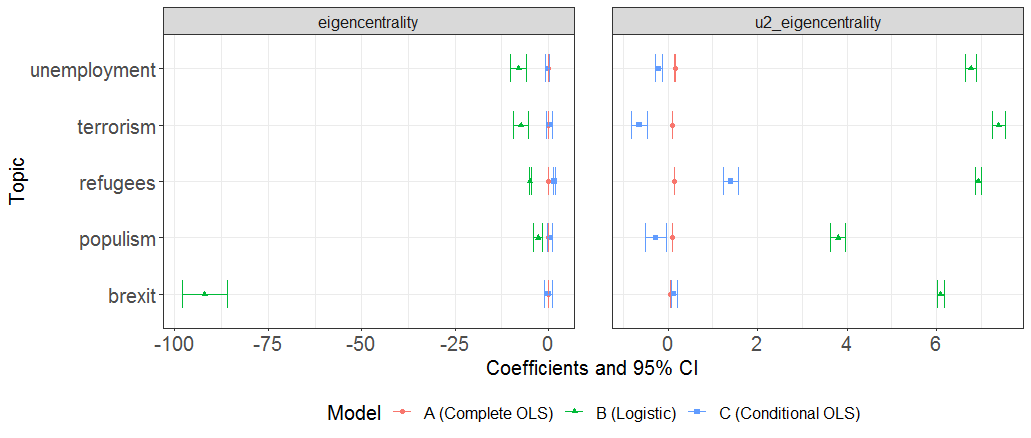
\includegraphics[width=\textwidth]{eigenxu2_eigen}
\caption*{\footnotesize$EC_{u1}$: We observe that the magnitude of effects varies between topic-networks in models B.\\$EC_{u2}$: We observe that the sign of the relationship varies between topic-networks in models C.}
\end{figure}

Figure \vref{eigenxu2eigencoeff} shows these graphs for $EC_{u1}$ and $EC_{u2}$. For instance, we observe that most of the $EC_{u2}$ coefficients' standard errors and their confidence intervals do not overlap (this is particularly evident in models B and C). When the error bars do not overlap, the difference between models' estimates may be significant\footnote{A statistical test should be performed to draw a conclusion.}. On the contrary, if error bars do overlap, we can conclude that the difference is not significant, and therefore that the paired coefficients do not statistically differ from each other. Thus, we infer that the $EC_{u2}$'s coefficients may statistically differ, and we speculate that this might be due to the intrinsic characteristics of the respective topic-network structures. In other words, structures with unique network characteristics – in terms of degree, centrality, and clustering – exist for different topics of discussion.
Similar graphs to Figure \ref{eigenxu2eigencoeff} for all variables can be found in the Appendix \vrefrange{model-a-coeff}{model-c-coeff}.

In summary, we find that the \textit{eigencentrality} of the target node ($EC_{u2}$) positively predicts the interaction and the number of interactions between nodes, regardless of the discussion topic. However, among those pairs of nodes that interacted, the direction of the effect of this variable on the number of interactions varies between topics. By contrast, the \textit{eigencentrality} of the source node ($EC_{u1}$) negatively influences the probability of interaction, but not the extent to which pairs of users interact with each other. Therefore, we conclude that the effect of \textit{eigencentrality} varies on whether it refers to the source or target node.

As regards the source's \textit{outdegree} ($OD_{u1}$), our data indicate that this positively influences both the probability of interactions and the number of interactions, regardless of the topic in discussion. However, given that two nodes have interacted, the direction of the effect of $OD_{u1}$ fluctuates between topics, although in a weaker way than the one of $EC_{u2}$. On the other hand, the target's \textit{outdegree} ($OD_{u2}$) negatively affects the probability of interaction between two nodes, regardless of the topic (except for \texttt{refugees}). However, among those pairs of users who interacted, the effect is overturned (positive and significant) for all topic-network structures.

Finally, we find that, regardless of the topic, both a highly clustered neighborhood of the source and target nodes ($CL_{u1}$ and $CL_{u2}$) positively influence the probability of interaction. Nevertheless, given that two nodes have interacted, highly dense clusters negatively affect the number of interactions between nodes (this is especially evident for \texttt{refugees}).

\clearpage % Multilm output table
\thispagestyle{SectionFirstPage}
\renewcommand{\arraystretch}{1.35}
\begin{sidewaystable}[!htbp]
  \centering
  \caption{Regression models A (Complete OLS) per topic.}
  \label{model-a}
  % Set table width
  \resizebox{0.7\width}{!}{\begin{tabular}{@{\extracolsep{0pt}}lccccc}
  \hline
   & \multicolumn{5}{c}{\textit{Dependent variable:}} \\
   \cline{2-6}
   \\[-2.8ex] & no. of interactions & no. of interactions & no. of interactions & no. of interactions & no. of interactions \\
   \\[-2.8ex] & (1) & (2) & (3) & (4) & (5)\\[+1.8ex]
   \hline
   & topic: \texttt{brexit} & topic: \texttt{populism} & topic: \texttt{refugees} & topic: \texttt{terrorism} & topic: \texttt{unemployment} \\
   \hline
   $OD_{u1}$ & .0003$^{***}$ & .003$^{***}$ & .001$^{***}$ & .001$^{***}$ & .001$^{***}$ \\
    & (0.00000) & (.0001) & (0.00000) & (.00002) & (.00002) \\
    & & & & & \\
   $EC_{u1}$ & .0002 & $-$.002 & .018$^{***}$ & $-$.001$^{*}$ & $-$.001 \\
    & (.0002) & (.002) & (.001) & (.001) & (.001) \\
    & & & & & \\
   $CL_{u1}$ & $-$.001$^{***}$ & $-$.001 & $-$.002$^{***}$ & $-$.001$^{*}$ & $-$.001$^{**}$ \\
    & (.0002) & (.002) & (.0003) & (.0004) & (.001) \\
    & & & & & \\
   $OD_{u2}$ & $-$0.00000 & $-$.001$^{***}$ & .0001$^{***}$ & $-$.0003$^{***}$ & $-$.0002$^{***}$ \\
    & (0.00000) & (.0001) & (0.00000) & (.00002) & (.00002) \\
    & & & & & \\
   $EC_{u2}$ & .058$^{***}$ & .100$^{***}$ & .151$^{***}$ & .103$^{***}$ & .155$^{***}$ \\
    & (.0002) & (.002) & (.001) & (.001) & (.001) \\
    & & & & & \\
   $CL_{u2}$ & $-$.002$^{***}$ & $-$.013$^{***}$ & $-$.017$^{***}$ & $-$.003$^{***}$ & $-$.005$^{***}$ \\
    & (.0002) & (.002) & (.0003) & (.0004) & (.001) \\
    & & & & & \\
   $constant$ & .001$^{***}$ & .006$^{***}$ & .003$^{***}$ & .002$^{***}$ & .002$^{***}$ \\
    & (.00001) & (.0002) & (.00004) & (.00003) & (.00004) \\
    & & & & & \\
   \hline
   Observations & 23,449,806 & 494,912 & 8,711,352 & 4,131,056 & 1,975,430 \\
   R$^{2}$ & .006 & .010 & .022 & .006 & .020 \\
   Adjusted R$^{2}$ & .006 & .010 & .022 & .006 & .020 \\
   Residual Std. Error & .032 (df = 23449799) & .130 (df = 494905) & .129 (df = 8711345) & .068 (df = 4131049) & .062 (df = 1975423) \\
   F Statistic & 22,474.450$^{***}$ (df = 6; 23449799) & 820.195$^{***}$ (df = 6; 494905) & 32,597.910$^{***}$ (df = 6; 8711345) & 4,091.516$^{***}$ (df = 6; 4131049) & 6,872.124$^{***}$ (df = 6; 1975423) \\
   \hline
   \multicolumn{1}{l}{\textit{Note:}}  & \multicolumn{5}{r}{$^{*}$p$<$0.1; $^{**}$p$<$0.05; $^{***}$p$<$0.01} \\
  \end{tabular}}
\end{sidewaystable}
\renewcommand{\arraystretch}{1.5}

\clearpage % Logit + multilm output table
\thispagestyle{SectionFirstPage} %if {empty} no page number either!
\renewcommand{\arraystretch}{1.4}
\begin{sidewaystable}[!htbp]
  \centering
  \small
  \caption{Regression models B (Logistic) and C (Conditional OLS) per topic.}
  \label{model-b-c}
  \resizebox{0.65\width}{!}{\begin{tabular}{@{\extracolsep{0pt}}l|cc|cc|cc|cc|cc}
  \hline % \hline doesn't need \\
   & \multicolumn{10}{c}{\textit{Dependent variable:}}\\
   \cline{2-11}
    & interacted & no. of interactions & interacted & no. of interactions & interacted & no. of interactions & interacted & no. of interactions & interacted & no. of interactions \\
 [+1ex]
  & & \textit{(conditional)} & & \textit{(conditional)} & & \textit{(conditional)} & & \textit{(conditional)} & & \textit{(conditional)} \\
   & \textit{logistic} & \textit{OLS} & \textit{logistic} & \textit{OLS} & \textit{logistic} & \textit{OLS} & \textit{logistic} & \textit{OLS} & \textit{logistic} & \textit{OLS} \\
 \\[-3.8ex] & (1) & (2) & (3) & (4) & (5) & (6) & (7) & (8) & (9) & (10)\\[+1.8ex]
 \cline{2-11}
 & \multicolumn{2}{c|}{topic: \texttt{brexit}} & \multicolumn{2}{c|}{topic: \texttt{populism}} & \multicolumn{2}{c|}{topic: \texttt{refugees}} & \multicolumn{2}{c|}{topic: \texttt{terrorism}} & \multicolumn{2}{c}{topic: \texttt{unemployment}} \\
 \hline
 $OD_{u1}$ & .079$^{***}$ & .004$^{***}$ & .302$^{***}$ & $-$.023 & .040$^{***}$ & .012$^{***}$ & .304$^{***}$ & $-$.068$^{***}$ & .219$^{***}$ & .017$^{***}$ \\
  & (.001) & (.001) & (.008) & (.016) & (.0003) & (.001) & (.005) & (.008) & (.004) & (.004) \\
  & & & & & & & & & & \\
 $EC_{u1}$ & $-$92.026$^{***}$ & $-$.001 & $-$2.738$^{***}$ & .415 & $-$4.875$^{***}$ & 1.587$^{***}$ & $-$7.341$^{***}$ & .277 & $-$7.961$^{***}$ & $-$.192 \\
  & (3.070) & (.500) & (.624) & (.377) & (.110) & (.174) & (1.014) & (.424) & (1.111) & (.294) \\
  & & & & & & & & & & \\
 $CL_{u1}$ & 4.018$^{***}$ & $-$.205 & .801$^{***}$ & .291 & .609$^{***}$ & $-$.881$^{***}$ & .663$^{***}$ & $-$.340$^{**}$ & .693$^{***}$ & $-$.196 \\
  & (.231) & (.234) & (.258) & (.347) & (.058) & (.250) & (.157) & (.172) & (.215) & (.149) \\
  & & & & & & & & & & \\
 $OD_{u2}$ & $-$.434$^{***}$ & .015$^{***}$ & $-$.613$^{***}$ & .069$^{**}$ & $-$.001$^{***}$ & .010$^{***}$ & $-$.703$^{***}$ & .066$^{***}$ & $-$.629$^{***}$ & $-$.006 \\
  & (.011) & (.003) & (.027) & (.030) & (.0002) & (.0005) & (.013) & (.012) & (.015) & (.006) \\
  & & & & & & & & & & \\
 $EC_{u2}$ & 6.101$^{***}$ & .136$^{***}$ & 3.800$^{***}$ & $-$.278$^{**}$ & 6.940$^{***}$ & 1.411$^{***}$ & 7.391$^{***}$ & $-$.638$^{***}$ & 6.775$^{***}$ & $-$.204$^{***}$ \\
  & (.037) & (.035) & (.085) & (.119) & (.032) & (.084) & (.072) & (.092) & (.062) & (.043) \\
  & & & & & & & & & & \\
 $CL_{u2}$ & $-$.069 & $-$.693 & $-$.541 & $-$.470 & .166$^{***}$ & $-$2.957$^{***}$ & $-$.347 & .218 & .485$^{*}$ & $-$.248 \\
  & (.545) & (.605) & (.363) & (.490) & (.046) & (.139) & (.237) & (.333) & (.273) & (.246) \\
  & & & & & & & & & & \\
 $constant$ & $-$9.227$^{***}$ & 1.383$^{***}$ & $-$7.022$^{***}$ & 2.465$^{***}$ & $-$7.306$^{***}$ & .885$^{***}$ & $-$8.113$^{***}$ & 2.109$^{***}$ & $-$7.644$^{***}$ & 1.398$^{***}$ \\
  & (.030) & (.014) & (.056) & (.071) & (.013) & (.032) & (.033) & (.033) & (.037) & (.020) \\
  & & & & & & & & & & \\
  \hline
  Observations & 23,449,806 & 9,146 & 494,912 & 1,346 & 8,711,352 & 13,846 & 4,131,056 & 4,452 & 1,975,430 & 3,296 \\
  R$^{2}$ &  & .008 &  & .009 &  & .201 &  & .028 &  & .018 \\
  Adjusted R$^{2}$ &  & .007 &  & .004 &  & .201 &  & .027 &  & .016 \\
  Pseudo R$^{2}$  & .165 &  & .181 &  & .268 &  & .175 &  & .227 & \\
  Log Likelihood & $-$67,633.010 &  & $-$7,636.007 &  & $-$75,693.210 &  & $-$28,825.970 &  & $-$18,883.490 &  \\
  Akaike Inf. Crit. & 135,280.000 &  & 15,286.010 &  & 151,400.400 &  & 57,665.950 &  & 37,780.990 &  \\
  Residual Std. Error &  & .784 (df = 9139) &  & 1.080 (df = 1339) &  & 2.330 (df = 13839) &  & .997 (df = 4445) &  & .611 (df = 3289) \\
  F Statistic &  & 12.133$^{***}$ (df = 6; 9139) &  & 1.917$^{*}$ (df = 6; 1339) &  & 581.356$^{***}$ (df = 6; 13839) &  & 21.444$^{***}$ (df = 6; 4445) &  & 9.946$^{***}$ (df = 6; 3289) \\
  \hline
  \multicolumn{1}{l}{\textit{Note:}} & \multicolumn{10}{r}{$^{*}$p$<$0.1; $^{**}$p$<$0.05; $^{***}$p$<$0.01} \\
  \end{tabular}}
\end{sidewaystable}
\renewcommand{\arraystretch}{1.5}
